\begin{abstract}
当每次试验必须先付款、成功收入又能继续使用时，完成学习所需的观测次数并不直接等于必须准备的启动资金。本文研究这一流动性约束如何影响行动选择。每个经营窗口有固定数量的单位奖励机会，投入强度连续可调，算法必须在余额允许的条件下学习并输出接近真实最优的投入。我们构造历史收入读数和若干暴露矩完全相同的环境，比较仅能观察首次成功与可以付费观察同一身份后续消息的两种权限。结果给出不同数量级的最低启动资金，以及首次反馈下资金与完成期限的匹配关系。重复消息的费用计入现金支出；允许不购买，因此更丰富的权限不会使最优策略变差。证明把完整日志的信息上界与实际付款路径联结，而非把平均亏损直接当作现金下界。一个固定机会池案例实际执行连续参数估计、逐窗付款、付费反馈和提前停止。结论限于已知模型模板下的基本极限；全部数值数据为合成，不代表真实市场验证。
\end{abstract}
\noindent\textbf{关键词：}序贯学习；启动资金；流动性约束；付费信息；停止规则

\section{研究问题：能否付到学会为止}
一个团队需要先购买搜索或处理资源，之后才可能取得收入。它希望通过试验判断应当采用多大的投入，但试验本身也在消耗余额。即使最后选择的行动足够好，余额也可能在得出答案之前耗尽。本文问的是：在不借款、收入可以回流的条件下，至少需要多少启动现金，才能可靠完成这项学习？

因此，本文的“融资”指完成学习所需的初始流动性，不涉及借贷利率、债务合约或企业资本结构。研究对象是经营和学习交织的起步阶段；数学困难在于信息与收入来自同一条随机路径，不能先算观测次数，再简单乘一个单价。

本文有两项主要结论。第一，是否能观察同一机会的后续消息，可以改变最低启动资金的数量级。第二，即使反馈权限固定，完成期限也会改变资金需求：较长时间允许小规模试验，减少经营亏损，但不能消除必要的信息等待风险。两项结论都包括必要下界和达到相同数量级的策略。

环境的结构先验很强：算法知道两个候选模型，或知道一条由连续参数决定的模型曲线，只是不知道哪一个参数为真。这里是在一个明确的学习任务中研究资金极限，并非从未知市场里发现任意交易策略。已有一套完全确定、无需再校准的行动时，本文的学习资金问题也就不再是同一任务。

\section{收入、付款时点和可观察的信息}
\subsection{每个窗口发生什么}
每个单位经营窗口重新产生 $K$ 个独立机会，$K$ 是已知固定整数。每个机会具有隐藏速度 $z>0$，独立服从概率分布 $\nu/K$，其中 $\nu$ 为总质量 $K$ 的非负有限测度。因而 $\nu(A)$ 是速度落在集合 $A$ 内的机会的期望数量，不是本窗实际机会组成。

开窗前选择连续投入 $q\in[0,1]$，预付资源费 $cq$。每个机会在窗内按速率 $qz$ 产生消息，首次消息带来 1 单位现金，以后消息只带来信息，不再支付奖励。因此
\begin{equation}\label{eq:income}
 P_\nu(q)=\int(1-e^{-qz})\,\nu(dz),\qquad
 f_\nu(q)=P_\nu(q)-cq.
\end{equation}
$P_\nu$ 是每窗口期望收入，$f_\nu$ 是未来执行时扣除资源费的期望利润。测试所购信息的费用另计。每窗首次成功数 $Y$ 服从 $\operatorname{Bin}(K,P_\nu(q)/K)$，实际现金不超过 $K$；机会池只在本窗口内使用，窗口间独立。

设 $C_{i-1}$ 为第 $i$ 窗开始前的余额，$J_i$ 为本窗购买的后续消息数，每条价格为 $\chi$。先检查
\begin{equation}\label{eq:cash}
 C_{i-1}\geq cq_i,
 \qquad C_i=C_{i-1}-cq_i+Y_i-\chi J_i.
\end{equation}
余额不足就不能开窗，也不能取得该窗日志。下文的具体购买策略从首次奖励中留存后续消息费用，保证费用可付。投入在看到本窗机会之前确定，不在窗中改动，也不借款或获得外部补贴。$q=0$ 不产生收入。

例如，余额为 2、每窗预付 1，连续两窗零收入后，就不能支付第三窗。即使第三窗原本可能取得 2 单位收入，也无法先用这笔未来现金付款。这说明最终账目或平均亏损不等于途中所需的启动资金。

\subsection{首次反馈和重复反馈是两种数据权限}
首次反馈包含全部首次成功消息及其精确时刻，窗末还知道机会目录和未成功的身份。同一身份的后续消息不提供给算法。重复反馈保留这些免费信息，并允许按条购买后续消息、随时免费取消。定理中的可行策略至多购买每个成功身份的 $d$ 条额外消息，固定价格满足
\[
 0\leq\chi<1/d.
\]
这样首奖励足以托管这些费用，每身份扣费后收入仍非负。正文不设强制入场费；若有可选的一次开通费，只给购买策略的充分准备金加一个固定量，不改变下文渐近指数。

首次反馈不是主动遗忘已经获得的数据，而是对可用数据的限制。去重报告或只保留首次事件的日志系统可能产生这样的区别，但本文没有校准具体业务。若某系统本来就免费提供完整日志，首次反馈只适合作为信息消融基准，没有必要真的关闭日志。

记两种权限下的最低启动资金为 $B^*_{\mathrm{first}}$ 与 $B^*_{\mathrm{repeat}}$。由于重复权限允许一条也不买，同一任务、同一精度和期限下必有
\begin{equation}\label{eq:inclusion}
 B^*_{\mathrm{repeat}}\leq B^*_{\mathrm{first}}.
\end{equation}
这只是弱排序；下文要说明某些任务中二者甚至具有不同的增长阶。表中的某个具体购买方案若更贵，也不能推翻式\eqref{eq:inclusion}。

\section{学会什么，以及至少需要多少现金}
\subsection{成功标准和困难环境}
给定允许利润损失 $\varepsilon>0$ 和失败概率 $0<\delta<1/2$，算法须对每个可能环境以至少 $1-\delta$ 的概率，同时做到：全程合法付款、有限时间输出 $\widehat q\in[0,1]$，且
\begin{equation}\label{eq:goal}
 \max_{0\leq q\leq1}f_\nu(q)-f_\nu(\widehat q)\leq\varepsilon.
\end{equation}
目标是接近真实模型的最优行动，不是取得信息集合下的保守保证。测试收入和信息费进入\eqref{eq:cash}；最后行动的精度按\eqref{eq:goal}评价，不等于测试全过程的总利润最大化。

设 $H$ 为最多允许的窗口数。$B_j^*(\varepsilon,H)$ 是权限 $j$ 下满足以上要求的初始余额下确界，允许随机、自适应选取 $q_i$ 和停止。$H=\infty$ 表示没有预设期限，成功仍须在有限时间给出答案。

本文构造的模型族带有难度参数 $\eta\downarrow0$ 和固定整数 $d\geq2$。两端模型的历史均值 $P(1),\ldots,P(n)$、总机会数 $K$ 及 $\int z^j\nu(dz)$（$j=2,\ldots,d$）完全相同；最优行动却不同。这里的矩是额外精确先验，不声称业务自然公开这些量。它们保持相同，是为了排除靠旧资料就能分辨环境的捷径。

在该族中取 $\varepsilon=\tau\eta^{2d-2}$，其中 $\tau>0$ 固定且足够小。算法知道整个候选模型和 $\eta$，不知道真实端点；扩展时不知道连续参数。结论是存在这样一组困难任务，不是每组读数或每个市场都有相同资金规律。

\subsection{反馈权限可以改变启动资金的增长阶}
\begin{theorem}[同一行动精度下的最低启动资金]\label{thm:capital}
对每个固定有限 $n\geq1$ 和 $d\geq2$，存在上述正机会模型族、固定整数 $K$ 及费用 $c>P(1)$，使全部公共信息在两端和充分小的 $\eta$ 上不变，且
\begin{equation}\label{eq:capital}
 B^*_{\mathrm{first}}(\varepsilon,\infty)\asymp\varepsilon^{-1/2},
 \qquad
 B^*_{\mathrm{repeat}}(\varepsilon,\infty)\asymp\varepsilon^{-\beta_d},
 \quad \beta_d=\max\left\{\frac14,\frac{d-2}{2d-2}\right\}.
\end{equation}
费用 $\chi$ 固定并满足上节合同。相同阶数还适用于两端凸组合形成的已知连续模型族，要求同一政策对每个参数均达到成功标准。
\end{theorem}

符号 $\asymp$ 表示上下相差固定正倍数，常数可依赖模型、$d,n,\delta,\tau,\chi$，但不依赖 $\varepsilon$。因此这不是有限尺度的确切报价，也不能在不同 $d$ 的不同模型之间直接比较金额。例如 $d=2$ 时，首次反馈为 $\varepsilon^{-1/2}$ 阶，重复反馈为 $\varepsilon^{-1/4}$ 阶；只有在精度足够高时，阶数差异才必然压过固定常数。

\noindent\textbf{为什么成立。}
构造加入少量高速机会，并调整慢机会的正权重，使旧资料不变。完整首次日志把高速信号混在背景里；同一身份的多次消息能更有效地暴露高速成分。信息下界迫使任何可靠政策完成一定量的试验，现金波动与经营亏损再给出必须持有的余额。具体低投入策略以相同阶数完成判断或连续参数估计，并留足付款准备，因此上下界匹配。附录\ref{app:construction}至\ref{app:upper}给出证明。

\noindent\textbf{对信息购买的含义。}
某些重复消息的价值不在于直接创造收入，而在于更早结束有风险的试验。定理已经计入按条收费，但没有解出一般消息的最优价格，也没有保证任何购买方式都划算。

\clearpage
\section{完成期限怎样改变资金需求}
\begin{theorem}[首次反馈的资金与期限关系]\label{thm:deadline}
沿用定理\ref{thm:capital}的同一个任务。记
\[
 H_0(\varepsilon)=\varepsilon^{-(2d-1)/(2d-2)}.
\]
存在固定正数 $c_\delta,C_\delta$：当 $H<c_\delta H_0$ 时，再多初始现金也不能可靠完成首次反馈任务；当 $H\geq C_\delta H_0$ 时，统一有
\begin{equation}\label{eq:frontier}
 B^*_{\mathrm{first}}(\varepsilon,H)
 \asymp\varepsilon^{-1/2}+\frac{\varepsilon^{-2}}H.
\end{equation}
重复反馈的最短可行期限为 $\varepsilon^{-d/(2d-2)}$ 阶；期限达到足够大的固定倍数后，可以用定理\ref{thm:capital}中的余额阶完成任务。
\end{theorem}

最短期限上下常数之间的准确分界未被求出。式\eqref{eq:frontier}的第一项是无法靠无限等待消除的现金风险；第二项来自期限紧张时较大投入造成的亏损。延长 $H$ 可以降低第二项，直到 $H$ 达到 $\varepsilon^{-3/2}$ 阶后，首次方案的启动余额已达其无期限最低阶。

\noindent\textbf{为什么成立。}
每窗能提供的信息有限，先给出最短期限。首次方案还需足够累计投入；若必须在 $H$ 窗完成，Jensen 不等式使平方投入和至少为累计投入平方除以 $H$。收入曲线的凹性把平方投入转为经营亏损，得到第二项。匹配策略在给定期限内使用固定小投入，既取得足够证据又预留现金波动准备。详见附录\ref{app:deadline}。

\noindent\textbf{对执行计划的含义。}
宽裕期限可以替代一部分启动资金，但不能把资金需求降为零。若项目连最短统计期限都无法满足，单纯增资也不能解决。式\eqref{eq:frontier}给的是指定任务中的量级关系；实际日历时间还须知道每个窗口多长，不能把窗口数直接当成天数。

$H$ 也不是购买条数。一个窗口包含 $K$ 个身份，每个身份可以产生多条消息；消息量随投入和随机命中而变。本文给出两种权限的资金比较及首次权限的期限关系，没有建立额外条数上限 $J$ 与最低资金的完整联合函数 $B^*(\varepsilon,H,J)$。

\section{一个有限机会池的完整执行案例}\label{sec:case}
本节在固定机会池上执行完整的学习与付款流程。每窗 $K=32$，速度节点为
\[
 z=(0.1,0.4,1,3,10,30).
\]
设两端概率权重为 $w_-,w_+$，由三个等式 $\sum w=1$、$\sum w(1-e^{-z})=0.5$、$\sum wz^2=25$ 定义，全部严格为正。未知参数 $\theta\in[-1,1]$，分布为 $w_\theta=(w_-+w_+)/2+\theta(w_+-w_-)/2$。精确权重方程见附录\ref{app:case}。这使所有参数共享 $K=32,P(1)=16,B_2=800$。

资源单价 $c=48$，行动精度 $\varepsilon=0.064$，期限 $H=4096$，每条额外消息费用 $\chi=0.005$，最多购买两条。两端最优行动约为 $0.000227$ 和 $0.091148$；任何不看新数据的公共行动，其最坏损失至少约 $0.483>\varepsilon$，所以该案例不能通过直接输出一个固定答案完成。

首次方案把首时刻分为 8 个等宽区间，加上失败，共 9 个类别。购买方案在同样的区间内再区分消息总数 1、2、至少 3，共 25 类；保留全部首次区间信息。实际计算的是这两个明确策略，不是两种权限下所有策略的有限尺度最优值。理论下界则已允许精确首次时刻。

两方案都估计连续 $\theta$。每个窗口先付款，再从同一组身份日志计入现金、消息费和统计量。在预定检查点构造参数置信区间，计算候选行动在整个区间上的最大利润损失；不超过 $\varepsilon$ 就停止，不继续等到 $H$。真实 $\theta$ 不用于决定停止时刻。

\begin{table}[H]\centering
\caption{同一任务、同一期限下的两种可执行方案}\label{tab:case}
\begin{tabular}{lrrrr}\toprule
方案 & 固定测试投入 & 充分准备金 & 验证用余额 & 最差联合成功率\\\midrule
首次反馈 & 0.03680 & 1889.18 & 317.87 & 99.95\%\\
购买重复消息 & 0.03261 & 1581.65 & 264.57 & 99.95\%\\\bottomrule
\end{tabular}
\end{table}

充分准备金由期望亏损和收入下尾公式计算，对整个参数区间有效，另有普通浮点计算误差；不是全策略最小资金。验证用余额来自与最终验证独立的试运行，金额较小，但只有验证网格上的经验证据。两列不能互换为同一种保证。投入在预先固定的 65 点菜单中选取，使充分准备金最小；没有使用最终验证样本调参。

本轮在 $\theta=-1,-0.75,\ldots,1$ 的 9 个条件、两种方案上各运行 2000 条有限余额路径，共 36000 条。一次联合成功同时要求合法付款、有限输出、真实行动损失达标、所有计算过的参数区间覆盖真值。最差组成功率为 99.95\%；对 18 组同时作单侧 95\% Clopper--Pearson 校正，每组成功率下界至少约 99.596\%。这些概率证据仅针对 18 个指定网格条件，不把有限网格当作整个连续参数区间的实验认证。

\begin{figure}[H]\centering
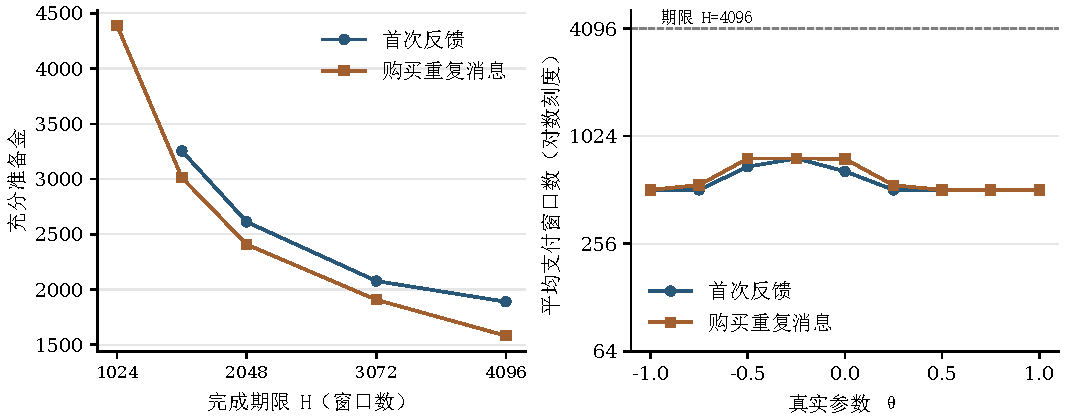
\includegraphics[width=\textwidth]{images/financing_case.pdf}
\caption{同一个有限任务。左图为不同期限下、给定投入菜单中的最低充分准备金，不是 $B^*$；没有点只表示该菜单未找到满足条件的方案。右图为最终验证实际支付的平均窗口数，对比期限 4096。收入、费用和估计都来自同一条逐窗路径。}\label{fig:case}
\end{figure}

购买方案的充分准备金低约 16.3\%，验证用余额低约 16.8\%，全部费用已经支付。两方案的平均停止窗口接近；本例的购买收益主要体现为用较低投入完成估计、减少现金需求，而非大幅缩短日历时间。这是两个具体方案的比较，不是付费权限有限尺度最优成本的精确差额。本例是固定有限模板，不是令 $\eta\to0$ 的指数实验，不能用这些金额拟合定理的渐近阶。

提前停止也确实影响付款。在 $\theta=-1$ 的亏损环境，把余额减为四分之一，或在已能给出答案后仍强制测到 4096 窗，两种方案的每项 1000 条独立控制路径都因停付失败。这个结果只针对上述控制条件；其他参数下收入可能支持继续试验，不能宣称所有继续经营都会破产。

程序直接按每窗 32 个独立身份的联合类别分布抽样，保留整条现金路径；没有用终点总收入替代中途付款。另有 80 万个身份的独立速度、指数首次时刻与后续消息生成检查，用于核对类别律。所有数据、图和表由本机重新运行程序生成，执行日志和源文件哈希随文保存。数值成功不认证附录中的资金下界，也不证明实际业务中一定有相同收益。

\section{用途、已有研究与限制}
学习受现金约束并非新问题。生存老虎机研究累计收益与破产风险\cite{riou}，资源约束最佳臂识别研究可靠选择\cite{li}，可补充背包模型允许资源回流\cite{replenish}。本文关注这些问题中的反馈机制：在相同精确公共约束、同一真实行动精度和预付合同下，完整首次日志与付费重复日志导致不同的最低资金阶；期限约束又把必要信息转化为额外经营亏损。上述结论需要同时处理身份内的消息依赖、现金回流和中途付款，不能仅由观测次数直接换算资金。

对实际项目，先识别需要追加学习的环境差异，再记录可观察的信息、付款时点和收入回流，才有条件讨论启动准备。付费消息是否值得购买，要看它能否缩短付费试验，而非只看增加了多少字段。若可以赊付、提前免费预览机会、跨窗复用机会或从外部获得安全收入，本文下界不能直接套用；这些制度会改变流动性约束本身。

模型仍假定已知模板、稳定机会分布和独立新生窗口。连续参数推广并未消除结构先验；任意未知市场中的最优采购、未知尺度下的学习，以及条数--期限--现金的完整联合设计仍未解决。每个合成窗口的规模有限，不等于已经证明真实市场的经济可行性。实际应用还需检验身份含义、重复消息机制、结算和费用合同。

\section*{代码与复现}
随文的\href{README.md}{复现入口}提供完整 LaTeX 源文件、程序、固定种子、结果和本机执行记录。本地链接需保留附件目录结构。当前没有公开仓库或 DOI；全部数据为合成，程序不连接账户、市场或交易系统。

\begingroup\small
\begin{thebibliography}{9}\setlength{\itemsep}{2pt}
\bibitem{riou} Riou, C., Honda, J., and Sugiyama, M. (2024).
The Survival Bandit Problem. arXiv:2206.03019v4.\par
\url{https://arxiv.org/abs/2206.03019}.
\bibitem{li} Li, Z. and Cheung, W. C. (2024). Best Arm Identification with Resource Constraints.
\emph{Proceedings of AISTATS}, PMLR 238, 253--261.\par
\url{https://proceedings.mlr.press/v238/li24c.html}.
\bibitem{replenish} Bernasconi, M., Castiglioni, M., Celli, A., and Fusco, F. (2023).
Bandits with Replenishable Knapsacks: the Best of both Worlds. arXiv:2306.08470.\par
\url{https://arxiv.org/abs/2306.08470}.
\bibitem{whitt} Whitt, W. (2007). Proofs of the martingale FCLT.
\emph{Probability Surveys}, 4, 268--302.\par
\href{https://doi.org/10.1214/07-PS122}{doi:10.1214/07-PS122}.
\end{thebibliography}\endgroup
